\section*{Data Exploration}

The data taken from the Colorado Department of Transportation has one row per accident, containing 295445 total observations. Heavy aggregation and preprocessing was done to prepare this data for modeling. In particular, these rows ended up being grouped by county and by season bringing the number of observations down to 256. That is 64 counties and 1 row for each season. 

\begin{table}[h!]
\centering
\begin{tabularx}{\textwidth}{|l|l|X|}
\hline
\rowcolor[HTML]{E7EAF6} 
\multicolumn{1}{|c|}{\textbf{Variable}} & \multicolumn{1}{c|}{\textbf{Data Type}} & \multicolumn{1}{c|}{\textbf{Description}}                     \\ \hline
County                                  & string                                 & Name of Colorado county                                        \\ \hline
Season                                  & factor         & Spring, Summer, Fall, Winter          \\ \hline
Deaths                                  & continuous numeric                     & \# of deaths per 100k residents                                \\ \hline
Injuries                                & continuous numeric & \# of injuries per 100k residents \\ \hline
Bad weather accidents                   & continuous numeric                     & \# of accidents in poor weather per 100k residents            \\ \hline
Median household income                 & continuous numeric & Median household income for county residents \\ \hline
Mean commuting time                     & continuous numeric                     & Mean commuting time for county residents (minutes)            \\ \hline
\end{tabularx}
\caption{Variables Used in the Analysis}
\label{tab:variables}
\end{table}

\subsection*{Response Variable: Injuries}

To start we will look at our response variable which represents the average number of injuries per 100k residents per year. \vspace{0.5cm}

\begin{center}
    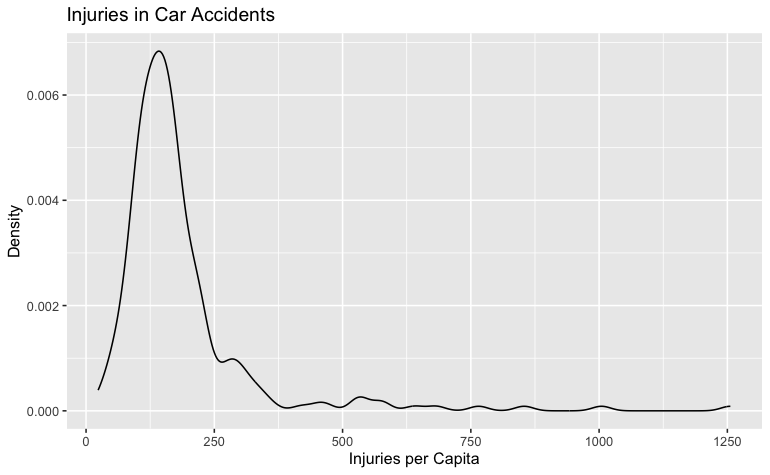
\includegraphics[width=0.8\columnwidth]{../presentation/presentation_images/injury_dist.png}
\end{center}

\pagebreak

It seems that, on average, a county in Colorado sees approximately 150 injuries in car accidents on any given season per year per 100 thousand residents. We can also see that the distribution of injuries appears log normal. We see most values hovering between 100 and 200 with a very long right tail. As we need our response variable to be normally distributed this immediately puts a log transformation into consideration. It is worth noting that a log transformation of the response variable does complicate model interpretation slightly and so should not be done without reason.

\begin{table}[h!]
\centering
\begin{tabular}{|l|r|r|r|r|r|r|}
\hline
\rowcolor[HTML]{E7EAF6} 
\multicolumn{1}{|c|}{\textbf{}} & \multicolumn{1}{c|}{Min} & \multicolumn{1}{c|}{1st Quartile} & \multicolumn{1}{c|}{Median} & \multicolumn{1}{c|}{Mean} & \multicolumn{1}{c|}{3rd Quartile} & \multicolumn{1}{c|}{Max} \\ \hline
Untransformed & 23.55 & 116.09 & 150.63 & 183.73 & 197.19 & 1255.83 \\ \hline
Transformed & 3.159 & 4.754 & 5.015 & 5.048 & 5.284 & 7.136 \\ \hline
\end{tabular}
\caption{Numerical summary of Injuries, with and without log transformation}
\end{table}

Instead of including a plot showing the transformed variable, I feel this numerical summary will suffice. The more extreme values have been pulled inline with the rest of our data which is shown by the mean not being as far from the median. The resulting density plot also does appear far more normal though is not included here. We will look at more evidence in the structural section of this report later. 

\subsection*{Predictor Variable Candidates}

\begin{table}[h!]
\centering
\begin{tabular}{|l|r|r|r|r|r|r|}
\hline
\rowcolor[HTML]{E7EAF6} 
\multicolumn{1}{|c|}{\textbf{Predictor}} & \multicolumn{1}{c|}{Min} & \multicolumn{1}{c|}{1st Quartile} & \multicolumn{1}{c|}{Median} & \multicolumn{1}{c|}{Mean} & \multicolumn{1}{c|}{3rd Quartile} & \multicolumn{1}{c|}{Max} \\ \hline
Deaths & 0 & 2.10 & 4.19 & 10.71 & 9.62 & 179.40 \\ \hline
Bad Weather Accidents & 0 & 28.33 & 51.37 & 93.43 & 97.23 & 904.07 \\ \hline
Income & 34578 & 56303 & 65976 & 70543 & 85228 & 139010 \\ \hline
Commute Time & 11.80 &  17.23 & 20.05 & 21.17 & 23.27 & 42.40 \\ \hline
\end{tabular}
\caption{Numerical summary of predictor candidates.}
\end{table}



